In this section, our goal is to establish properties of Hilbert spaces and kernel functions that can be used to modify the PCA algorithm.
To begin, we will briefly cite some definitions and results from analysis \cite{kreyszig1991introductory}, \cite{rudin1987real} and matrix theory \cite{horn2013matrix}.

\begin{definition}[Definite matrix]
    \label{def:definite-matrix}
    \cite{horn2013matrix}
    Let \(A\) be an \(n \times n\) matrix over the real numbers having the form
\begin{equation}
    A = \begin{bmatrix}
        a_{11} & a_{12} & \cdots & a_{1n}\\
        a_{21} & a_{22} & \cdots & a_{2n}\\
        \vdots & \vdots & \ddots & \vdots\\
        a_{n1} & a_{n2} & \cdots & a_{nn}\\
    \end{bmatrix} = [a_{ij}].
\end{equation}
The \textit{transpose} of \(A\) is \(A^\top = [a_{ji}]\).
We say that \(A\) is \textit{symmetric} whenever \(A = A^\top\).
A symmetric matrix \(A\) is
\begin{enumerate}
    \item \label{part:positive-definite-matrix}
    \textit{positive definite} if \(x^\top A x > 0\), for all nonzero \(x \in \RR^n\), or
    \item \label{part:positive-semidefinite-matrix}
    \textit{positive semidefinite} if \(x^\top A x \geq 0\), for all \(x \in \RR^n\).
\end{enumerate} 
% \begin{align}
%     x^\top A x &> 0, \quad \text{for all nonzero \(x \in \RR^n\)}
%     \intertext{and is \textit{positive semidefinite} if}
%     x^\top A x &\geq 0, \quad \text{for all \(x \in \RR^n\)}.
% \end{align}
Negative (semi)definite matrices can be defined in a similar fashion.
A matrix is \textit{definite} if it is either positive semidefinite or negative semidefinite.
Otherwise, \(A\) is an \textit{indefinite matrix}.

Be aware that some authors use the terms positive definite (\(>\)) and nonnegative definite (\(\geq\)).
Other authors use the modifier \textit{strict} as in strict positive definite (\(>\)) and positive definite (\(\geq\)).
\end{definition}

\begin{definition}[Inner product]
    \label{def:inner-product}
    \cite{small1994hilbert} % page 10
    % begin macros
\def\innerprod{\ipt{\cdot, \cdot}}
\def\qand{\quad\text{and}\quad}
% end macros
% 
Let \(\innerprod : \X \times \X \to \RR\) be a function defined on the vector space \(\X\).
Then \(\innerprod\) is an \textit{inner product} if the following properties hold for all \(x, y, z \in \X\) and \(\alpha, \beta \in \RR\):
\begin{enumerate}
    \item %Symmetry:
    \(\ipt{x,y} = \ipt{y,x}\);
    \hfill (symmetry)
    \item %Bilinearity:
    \(\ipt{\alpha x + \beta y, z} = \alpha \ipt{x, z} + \beta \ipt{y, z}\);
    \hfill (bilinear)
    \item %Positive definiteness:
    \(\ipt{x,x} \geq 0\) and \(\ipt{x,x} = 0\) if and only if \(x = 0\).
    \hfill (positive definite)
\end{enumerate}
Note that linearity in the first argument with symmetry implies that the inner product is bilinear (linear in both arguments).
Since inner products are positive definite, they induce a norm \(\| \cdot \| : \X \to \RR\) and metric \(d : \X \times \X \to \RR\) such that
\begin{equation}
    \|x\| = \sqrt{\langle x, x \rangle}
    \qand
    d(x,y) = \|x - y\|.
\end{equation}
An \textit{inner product space}, \textit{normed space}, and \textit{metric space} are vector spaces along with an inner product, norm, and metric, respectively.
It follows that an inner product space is also a normed space and a metric space.
Then the induced norm has the following properties for all \(x, y \in \X\) and \(\alpha \in \RR\):
\begin{enumerate}
    \item \(\|\alpha x\| = |\alpha| \|x\|\);
    \item \(\|x\| \geq 0\) and \(\|x\| = 0\) if and only if \(x = 0\);
    \item \(\|x + y \| \leq \|x\| + \|y\|\);
    \hfill (triangle inequality)
    \item \(\langle x, y \rangle^2 \leq \|x\| \|y\|\).
    \hfill (Cauchy-Schwarz inequality)
\end{enumerate}
\end{definition}

\begin{example}
    \label{eg:dot-product}
    The \textit{Euclidean inner product} (or \textit{dot product}) is the function \(\langle \cdot, \cdot \rangle : \RR^n \times \RR^n \to \RR\) such that
\begin{equation}
    \langle x, y \rangle = \sum_{i=1}^{n} x_i y_i = x^\top y,
\end{equation}
for all \(x = [x_i], y = [y_i] \in \RR^n\).
Sometimes we write \(x \dotprod y\) to mean the Euclidean inner product.
This induces the \textit{Euclidean norm}
\begin{equation}
    \|x\| = \sqrt{\sum_{i=1}^{n} x_i^2}
\end{equation}

% Checking that this is an inner product:
% \begin{enumerate}
%     \item \(\begin{aligned}[t]
%         \langle x, y \rangle = \sum_{i=1}^{n} x_i y_i = \langle y, x \rangle
%     \end{aligned}\);
%     \item \(\begin{aligned}[t]
%         \langle \alpha x + \beta y, z \rangle
%         &= \sum_{i=1}^{n} (\alpha x_i + \beta y_i) z_i\\
%         &= \alpha \sum_{i=1}^{n} x_i z_i + \beta \sum_{i=1}^{n} y_i z_i
%         = \alpha \langle x, z \rangle
%         + \beta \langle y, z \rangle;
%     \end{aligned}\)
%     \item Let \(x \neq 0\).
%     Then there is some nonzero \(x_a \in \{x_1, x_2, \dots, x_n\}\) such that
%     \(\langle x, x \rangle = \sum_{i=1}^{n} x_i^2 \geq x_a^2 > 0\).
%     Also, \(\langle 0, 0 \rangle = 0\).
% \end{enumerate}
\end{example}

\begin{definition}[Hilbert space]
    \label{def:hilbert-space}
    \cite{kreyszig1991introductory}
    A metric space is \textit{complete} if the limit of every Cauchy sequence is in the space.
A complete normed space is called a \textit{Banach space}.
A complete inner product space \(\H\) is called a \textit{Hilbert space}.
We sometimes denote the inner product and norm of \(\H\) as \(\ipt{\cdot, \cdot}_H\) and \(\|\cdot\|_{\H}\) to avoid ambiguity.

% Kreyszig, Definition 1.3.5, page 21
A Hilbert space is said to be \textit{separable} if it contains a dense countable subset.
% Kreyszig, Theorem 3.6.4, page 171
It can be shown that a Hilbert space is separable if and only if it has a countable orthonormal basis.

% Kreyszig, page 173
\def\L{\hilbert{L}}
Two real Hilbert spaces \(\H\) and \(\L\) are said to be \textit{isomorphic} if there is a linear bijection \(T : \H \to \L\) such that
\begin{equation}
    \label{eqn:hilbert-space-isomorphism}
    \ipt{x,y}_{\H} = \ipt{Tx, Ty}_{\L},
\end{equation}
for every \(x, y \in \H\).
In \cite{kreyszig1991introductory}, Kreyszig shows that two Hilbert spaces are isomorphic if and only if they have the same dimension.
% Theorem 3.6.5, page 173
If \(\H\) is an inner product space that is not complete, then it can be extended to a Hilbert space by completion.
The completion of an inner product space is denoted as \(\overline{\H}\) and is unique up to isomorphism.
\end{definition}

The following example demonstrates a useful property of separable Hilbert spaces.

\begin{example}
    \label{eg-l2-hilbert-space}
    \cite{rudin1987real}
    % Rudin, pages 84-85
Let \(A\) be a nonempty index set.
The space of square-summable indexed families is defined as
\begin{equation}
    \label{eqn:l2-space}
    \ell^2(A) = \left\{
        x : A \to \RR \;\middle\vert\; \sum_{a \in A} x_a^2 < \infty
    \right\}.
\end{equation}
Given the inner product
\begin{equation}
    \label{eqn:l2-inner-product}
    \langle x, y \rangle = \sum_{a \in A} x_a y_a,
\end{equation}
\(\ell^2(A)\) is a Hilbert space.
Moreover, \(\ell^2(A)\) is separable if and only if \(A\) is countable.
It follows that the sequence space \(\ell^2 = \ell^2(\NN)\) is the separable Hilbert space of square-summable sequences.
Due to the Riesz-Fischer theorem, every infinite-dimensional Hilbert space is isomorphic to \(\ell^2\).
\end{example}

TODO: Define Hilbert space dual

\begin{definition}[Gram matrix]
    \label{def:gram-matrix}
    \cite{horn2013matrix}
    Let \(x_1, x_2, \dots, x_n \in \X\) for some inner product space \(\X\) equipped with \(\langle \cdot, \cdot \rangle\).
We say \(G\) is a \textit{Gram matrix} (or \textit{Gramian}) for the sequence of vectors \(x_1, x_2, \dots, x_n\) with respect to \(\langle \cdot, \cdot \rangle\) if \(G = \begin{bmatrix}
    \langle x_i, x_j \rangle
\end{bmatrix}_{ij}\).
\end{definition}

\begin{example}
    \label{eg:gram-matrix}
    % TODO: Clean up gram matrix example.

% begin macros
\def\v{\mathbf{v}}
% end macros
% 
Consider the vectors in \(\RR^3\):
\begin{align*}
    \v_1 &=
    \begin{bmatrix}
        v_{11} \\ v_{21} \\ v_{31}
    \end{bmatrix},&
    \v_2 &=
    \begin{bmatrix}
        v_{12} \\ v_{22} \\ v_{32}
    \end{bmatrix},&
    \v_3 &=
    \begin{bmatrix}
        v_{13} \\ v_{23} \\ v_{33}
    \end{bmatrix},&
    \v_4 &=
    \begin{bmatrix}
        v_{14} \\ v_{24} \\ v_{34}
    \end{bmatrix}.
\end{align*}
The Gram matrix for these vectors is
\begin{align*}
    G = \begin{bmatrix}
        \v_1^\top \v_1 & \v_1^\top \v_2 & \v_1^\top \v_3 & \v_1^\top \v_4\\[3pt]
        \v_2^\top \v_1 & \v_2^\top \v_2 & \v_2^\top \v_3 & \v_2^\top \v_4\\[3pt]
        \v_3^\top \v_1 & \v_3^\top \v_2 & \v_3^\top \v_3 & \v_3^\top \v_4\\[3pt]
        \v_4^\top \v_1 & \v_4^\top \v_2 & \v_4^\top \v_3 & \v_4^\top \v_4\\
    \end{bmatrix}.
\end{align*}
If \(V\) is a matrix whose columns are \(\v_1\), \(\v_2\), \(\v_3\), \(\v_4\), then we can write \(G = V^\top V\).
\end{example}

\begin{theorem}
    \label{thm:gram-psd}
    \cite{horn2013matrix}
    A matrix \(G\) is a Gram matrix if and only if \(G\) is positive semidefinite.
\end{theorem}
\begin{proof}
    (\(\Rightarrow\))
Suppose \(G\) is the Gram matrix of \(x_1, x_2, \dots, x_n\) with respect to \(\langle \cdot, \cdot \rangle\).
Let \(c_1, c_2, \dots, c_n \in \RR\).
Then \(G\) is positive semidefinite because
\begin{align}
    \sum_{i=1}^{n} \sum_{j=1}^{n} c_i c_j \langle x_i, x_j \rangle
    = \left\langle
        \sum_{i=1}^{n} c_i x_i, \sum_{j=1}^{n} c_j x_j
    \right\rangle
    = \left\|
        \sum_{i=1}^{n} c_i x_i
    \right\|^2
    \geq 0.
\end{align}

(\(\Leftarrow\))
Suppose \(G\) is positive semidefinite.
Then \(G\) can be factored as \(G = B^\top B\).
Let \(b_1, b_2, \dots, b_n\), be the columns of \(B\).
Then \(G = [b_i^\top b_j]_{ij}\).
Hence \(G\) is the Gram matrix of \(b_1, b_2, \dots, b_n\) with respect to the dot product.
\end{proof}

\begin{theorem}
    \label{thm:gram-pd-iff-lin-indep}
    \cite{horn2013matrix}
    A Gram matrix \(G\) of \(x_1, x_2, \dots, x_n\) is positive definite if and only if \(x_1, x_2, \dots, x_n\) are linearly independent.
\end{theorem}
\begin{proof}
    % TODO: Prove that a Gram matrix is positive semidefinite iff its columns are linearly independent.

% This proof is in Horn

\end{proof}

\begin{definition}[Symmetric bilinear form]
    \label{def:symmetric-bilinear-form}
    A \textit{symmetric bilinear form} is a map \(k : \X \times \X \to \RR\) over a vector space \(\X\) such that, for all \(x,y,z \in \X\), \(\alpha, \beta \in \RR\),
\begin{enumerate}
    \item \(k(x,y) = k(y,x)\) and
    \hfill (symmetry)
    \item \(k(\alpha x + \beta y, z) = \alpha k(x,z) + \beta k(y,z)\).
    \hfill (bilinear)
\end{enumerate}
\end{definition}

This can be thought of as a generalization of an inner product which is symmetric and bilinear, but not necessarily positive definite.

\begin{example}
    \label{eg:symmetric-bilinear-form}
    If \(U = \{u_1, u_2, \dots, u_n\}\) is a basis for \(\X\), then we can define a matrix \(K = \begin{bmatrix}
    k(u_i, u_j)
\end{bmatrix}_{ij}\).
Clearly, \(K\) is symmetric since \(k(u_i, u_j) = k(u_j, u_i)\).
Let \(v = \sum_{i=1}^n \alpha_i u_i\) and \(w = \sum_{i=1}^n \beta_i u_i\) be vectors with respect to \(U\) and let \(x = [\alpha_i]_{i=1}^n\) and \(y = [\beta_i]_{i=1}^n\).
Then
\begin{equation}
    \label{eqn:bilinear-form-representation}
    k(v,w)
    = k\left(\sum_{i=1}^n \alpha_i u_i, \sum_{j=1}^{n} \beta_j u_j\right)
    = \sum_{i=1}^n \sum_{j=1}^{n} \alpha_i \beta_j k\left(u_i, u_j\right)
    = x^\top K y.
\end{equation}
If \(K = I\), then \(v = x\), \(w = y\), and \(k(v,w) = v^\top w\) is simply the dot product.
Otherwise, if \(K\) is positive semidefinite, then \(K = B^\top B\) implies
\begin{equation}
    \label{eqn:bilinear-form-dot-product}
    k(v,w) = x^\top B^\top B y = (Bx)^\top (By)
\end{equation}
In this case, \(k(v,w)\) is just the dot product after the transformation under \(B\).
Notice that if \(U\) is merely a subset of \(\X\), then \(v\) and \(w\) no longer have unique representations, but \cref{eqn:bilinear-form-representation,eqn:bilinear-form-dot-product} are still valid for all \(v, w \in \lspan U\).

We say that \(k\) is \textit{positive semidefinite} if \(K = [k(u_i, u_j)]_{ij}\) is a positive semidefinite matrix for any finite subset \(U = \{u_1, u_2,\dots, u_n\} \subseteq \X\).
Then \(K\) is a Gram matrix with respect to some set of transformed vectors related to \(U\) and some inner product related to \(k\).
In the next subsection, we will show that \(k\) still corresponds to some inner product even if \(k\) is not bilinear.

\end{example}

\subsection{Kernels}
\label{sub:kernels}
The development of \textit{kernel functions} can be traced back to the beginning of the twentieth century when David Hilbert and James Mercer were studying integral equations \cite{hofmann2008kernel}.
Hilbert proved some important results in \cite{hilbert1912grundzüge} about the eigenvalues of an integral operator whose kernel function is of \textit{definite} type.
Expanding on Hilbert's work, Mercer provided the necessary conditions in \cite{mercer1909xvi} that allow a kernel function to be written in terms of the eigenvalues and eigenfunctions of the integral operator.
This result became known as Mercer's theorem.
See \Cref{sec:mercers-theorem}.
A simplified version of Mercer's theorem states that a kernel function can be written as an inner product in a higher-dimensional space.

Hilbert space theory and Mercer's theorem led to a number of advances in functional analysis over the next few decades.
Notably, in 1950, Nachman Aronszajn introduced reproducing kernel Hilbert spaces in \cite{aronszajn1950theory}.
This work expanded on Mercer's theorem and shows that a kernel generates a Hilbert space whose inner product agrees with the kernel.

Later, the work of Mercer and Aronszajn inspired the application of kernels in machine learning.
A \textit{kernel method} is an adaptation of a machine learning algorithm that replaces a dot product with a kernel function.
The earliest research involving kernel methods was in 1964 by Mark Aizerman et al. \cite{aizerman1964theoretical}.
In the 1990s, Bernhard Sch\"olkopf et al. used Aizerman's technique to develop kernel PCA and suggested the kernel trick could work in other cases too.
In \Cref{sec:kernel-pca}, we will look at the kernel method applied to the PCA algorithm.
For now, we will examine the mathematics behind kernel methods.

\begin{definition}[Kernel]
    \label{def:kernel}
    \cite{rudin2020notes}
    Let \(k : \X \times \X \to \RR\) be defined on a nonempty set \(\X\).
Similar to the Gram matrix, define a \textit{kernel matrix} for a set of vectors \(\{x_1, x_2, \dots, x_n\} \subseteq X\) with respect to \(k(\cdot, \cdot)\) as \(K = [k(x_i,x_j)]_{ij}\).
Then \(k\) is a \textit{kernel function} (or just \textit{kernel}) if the following hold:
\begin{enumerate}
    \item \(k(x,y) = k(y,x)\), for all \(x,y \in \X\) and
    \hfill (symmetry)
    \item any kernel matrix \(K\) generated by \(k\) is positive semidefinite.
\end{enumerate}
\end{definition}

We can easily show some properties that kernels have in common with inner products.

\begin{lemma}
    \label{lem:properties-of-kernels}
    \cite{rudin2020notes}
    Let \(k\) be a kernel.
Then the following hold:
\begin{enumerate}
    \item \label{itm:properties-of-kernels-psd}
    \(k(x,x) \geq 0\) for all \(x \in \X\) and
    \hfill (positive semidefinite)
    \item \label{itm:properties-of-kernels-csi}
    \(k(x,y)^2 \leq k(x,x) k(y,y)\).
    \hfill (Cauchy-Schwarz inequality)
\end{enumerate}
\end{lemma}
\begin{proof}
    Let \(x,y \in \X\).
\begin{enumerate}
    \item The \(1 \times 1\) kernel matrix \([k(x,x)]\) is positive semidefinite.
    So, \(k(x,x) \geq 0\).
    \item The \(2 \times 2\) kernel matrix
    \begin{equation}
        K = \begin{bmatrix}
            k(x,x) & k(x,y) \\ k(y,x) & k(y,y)
        \end{bmatrix}
    \end{equation}
    is positive semidefinite.
    Let \(v = \begin{bmatrix}
        k(y,y) \\ -k(x,y)
    \end{bmatrix}\).
    Then
    \begin{align}
        0 &\leq v^\top K v\\
        &= \begin{bmatrix}
            k(y,y) \\ -k(x,y)
        \end{bmatrix}^\top
        \begin{bmatrix}
            k(x,x)k(y,y) - k(x,y)^2 \\ 0
        \end{bmatrix}
        \notag\\
        % &= k(y,y) \left[
        %     k(y,y) k(x,x) - k(x,y)^2
        % \right]
        % \notag\\
        % &\qquad - k(x,y) \left[
        %     k(y,y) k(y,x) - k(x,y) k(y,y)
        %     \right]
        % \notag\\
        &= k(y,y) \left[
            k(x,x)k(y,y) - k(x,y)^2
        \right].
        \notag
    \end{align}
    Then \(v^\top K v \geq 0\) implies \(k(x,y)^2 \leq k(x,x) k(y,y)\).
    \qedhere
\end{enumerate}
\end{proof}

\begin{definition}[Feature map]
    \label{def:feature-map}
    \cite{hofmann2008kernel}
    Let \(\X\) be a nonempty set and let \(\RR^{\X}\) be the vector space of real-valued functions on \(\X\).
% For example, any function \(f : \X \to \RR\) is in \(\RR^{\X}\).
A \textit{feature map} is a function \(\Phi : \X \to \H\) for some subspace \(\H \subseteq \RR^{\X}\).
In this context, \(\H\) is referred to as the \textit{feature space} and its elements \(\Phi(x) \in \H\) are called \textit{features}.
\end{definition}

Starting with a kernel \(k : \X \times \X \to \RR\), we want to construct a feature map \(\Phi : \X \to \H\) and inner product \(\ipt{\cdot, \cdot} : \H \times \H \to \RR\) which satisfies
\begin{equation}
    \label{eqn:kernel-inner-product-1}
    k(x,y) = \ipt{\Phi(x), \Phi(y)},
\end{equation}
for all \(x, y \in \X\).
Then the linear span of \(\Phi(\X) = \{\Phi(x) \mid x \in \X\}\) will be an inner product space.
Since inner product spaces can be completed, we can make this a Hilbert space.
See \Cref{fig:kernel-map-diagram}.

\begin{figure}
    \centering
    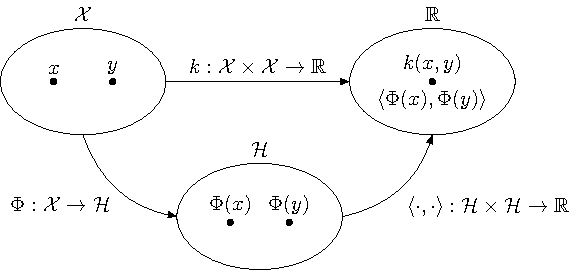
\includegraphics[]{figs/fig-kernel-map-diagram}
    \caption{Kernel map diagram.}
    \label{fig:kernel-map-diagram}
\end{figure}

\paragraph{Constructing a feature map.}
\def\Ho{H_0}
\def\iptHo#1{\ipt{#1}_{\Ho}}

Consider the map\footnote{
    Here, \(\Phi : \X \to (\X \to \RR)\) is just the \textit{curried} form of the binary function \(k : \X \times \X \to \RR\).
    For example, \(\{k(x, \cdot) \mid x \in \X\}\) describes a set of unary functions curried from the binary function \(k\).
} \(\Phi(x) = k(x, \cdot)\), for all \(x \in \X\).
Note that by the symmetry of \(k\), we can write \(\Phi(x) = k(x, \cdot) = k(\cdot, x)\).
Taking the linear span of \(\Phi(\X)\) gives us
\begin{equation}
    \Ho = \lspan \Phi(\X)
    = \left\{
        f = \sum_{i=1}^{n} \alpha_i k(x_i, \cdot)
        \;\middle|\;
        \begin{aligned}
            \forall n &\in \NN,\\
            x_1, x_2, \dots, x_n &\in \X,\\
            \alpha_1, \alpha_2, \dots, \alpha_n &\in \RR
        \end{aligned}
    \right\},
\end{equation}
which forms a subspace of \(\RR^{\X}\).
By \Cref{def:feature-map}, \(\Ho\) is a feature space.

\paragraph{Constructing an inner product.}

Let \(f,g \in \Ho\).
Then there exist \(n, m \in \NN\), \((\alpha_i)_{i=1}^n\), \((\beta_j)_{j=1}^m\), \((x_i)_{i=1}^n\), \((y_j)_{j=1}^m\) such that
\begin{equation}
    \label{eqn:function-linear-combo}
    f = \sum_{i=1}^{n} \alpha_i k(x_i, \cdot)
    \quad\text{and}\quad
    g = \sum_{j=1}^{m} \beta_j k(y_j, \cdot).
\end{equation}
Define \(\iptHo{\cdot, \cdot} : \Ho \times \Ho \to \RR\) as
\begin{equation}
    \label{eqn:pre-hilbert-inner-product}
    \iptHo{f, g} 
    = \sum_{i=1}^{n} \sum_{j=1}^{m} \alpha_i \beta_j k(x_i, y_j).
\end{equation}
Letting \(m=1\), \(\beta_1=1\), \(y_1 = y\) in \cref{eqn:function-linear-combo,eqn:pre-hilbert-inner-product}, then \(g = k(y,\cdot)\).
This shows that \(k\) has the \textit{reproducing property}
\begin{equation}
    \label{eqn:reproducing-property}
    \iptHo{f, k(y, \cdot)} = \sum_{i=1}^{n} \alpha_i k(x_i, y) = f(y),
\end{equation}
for all \(y \in \X\).
Similarly, letting \(n=1\), \(\alpha_1=1\), \(x_1=x\), we have
\begin{equation}
    \label{eqn:kernel-is-inner-product}
    k(x,y) = \iptHo{k(x,\cdot), k(y,\cdot)} = \iptHo{\Phi(x), \Phi(y)},
\end{equation}
for all \(x,y \in \X\).
Now we will show that \(\iptHo{\cdot, \cdot}\) is an inner product.
\begin{enumerate}
    \item Since \(k\) is symmetric, we have
    \begin{equation}
        \iptHo{f, g}
        = \sum_{i=1}^{n} \sum_{j=1}^{m} \alpha_i \beta_j k(x_i, y_j)
        = \sum_{j=1}^{m} \sum_{i=1}^{n} \beta_j \alpha_i k(y_j, x_i)
        = \iptHo{g, f}.
    \end{equation}
    \item By rearrangement, \cref{eqn:pre-hilbert-inner-product} becomes
    \begin{equation}
        \iptHo{f, g}
        % = \sum_{i=1}^{n} \sum_{j=1}^{m} \alpha_i \beta_j k(x_i, y_j)
        = \sum_{j=1}^{m} \beta_j \sum_{i=1}^{n} \alpha_i k(x_i, y_j)
        = \sum_{j=1}^{m} \beta_j f(y_j).
    \end{equation}
    Then for all \(f_1, f_2 \in \lspan \Phi(\X)\) and \(\alpha, \gamma \in \RR\),
    \begin{align}
            \iptHo{\alpha f_1 + \gamma f_2, g}
            &= \sum_{j=1}^{m} \beta_j (\alpha f_1 + \gamma f_2)(y_j) \\
            &= \alpha \sum_{j=1}^{m} \beta_j f_1(y_j) + \gamma \sum_{j=1}^{m} \beta_j f_2(y_j)
            \notag\\
            &= \alpha \iptHo{f_1, g} + \gamma \iptHo{f_2, g}.
            \notag
    \end{align}
    \item Since \(k\) is positive semidefinite, by \Cref{lem:properties-of-kernels} \cref{itm:properties-of-kernels-psd}
    \begin{equation}
        \iptHo{f,f}
        = \sum_{i=1}^{n} \sum_{j=1}^{n} \alpha_i \alpha_j k(x_i, x_j)
        % = a^\top K a
        \geq 0.
    \end{equation}
    Now let \(f_1, f_2, \dots, f_p\) be functions and \(\gamma_1, \gamma_2, \dots, \gamma_p \in \RR\).
    Then by bilinearity,
    \begin{equation}
        \sum_{i=1}^{p} \sum_{j=1}^{p} \gamma_i \gamma_j \iptHo{f_i, f_j}
        = \iptHo{\sum_{i=1}^{p} \gamma_i f_i, \sum_{j=1}^{p} \gamma_j f_j}
        \geq 0.
    \end{equation}
    Thus, \(\iptHo{\cdot, \cdot}\) is a kernel.
    Then by \cref{eqn:reproducing-property} and \Cref{lem:properties-of-kernels} \cref{itm:properties-of-kernels-csi},
    \begin{equation}
        f(x)^2 = \iptHo{f, k(x, \cdot)}^2 \leq \iptHo{f,f} \iptHo{k(x, \cdot), k(x, \cdot)},
    \end{equation}
    for all \(x \in \X\).
    If \(\iptHo{f,f} = 0\), then \(f(x)^2 = 0\) implies \(f = 0\).
\end{enumerate}

\paragraph{Constructing a Hilbert space.}
\def\iptH#1{\ipt{#1}_{\H}}
Now that we know \(\iptHo{\cdot, \cdot}\) is an inner product, \(\Ho\) is an inner product space.
By \cite{kreyszig1991introductory}, this can be completed with respect to the induced metric.
Then
\begin{equation}
    \label{eqn:complete-feature-space}
    \H
    % = \overline{\Ho}
    = \overline{\lspan \Phi(\X)}
    = \overline{\lspan\{k(x, \cdot) \mid x \in \X\}}
\end{equation}
is a Hilbert space with inner product \(\iptH{\cdot, \cdot} : \H \times \H \to \RR\).
Since \(\H\) contains all its limit points, functions in this space have the form
the sequences \((\alpha_i)_{i=1}^\infty\) and \((x_i)_{i=1}^\infty\) determine a function \(f \in \H\) such that
\begin{equation}
    f = \sum_{i=1}^{\infty} \alpha_i k(x_i, \cdot),
\end{equation}
provided the series converges.

\begin{definition}[Reproducing kernel Hilbert space]
    \label{def:reproducing-kernel-hilbert-space}
    \cite{hofmann2008kernel}
    Let \(\H\) be a Hilbert space of functions \(\X \to \RR\) on some nonempty set \(\X\).
Then \(\H\) is a \textit{reproducing kernel Hilbert space} (RKHS) if there exists a function \(k : \X \times \X \to \RR\) such that for all \(f \in \H\) and \(x \in \X\),
\begin{enumerate}
    \item \(f(x) = \ipt{f, k(x,\cdot)}\) and
    \hfill (reproducing property)
    \item \(\H = \overline{\lspan\{k(x,\cdot) \mid x \in \X\}}\).
    \hfill (spanning property)
\end{enumerate}
\end{definition}

Fix \(y \in \X\) and treat \(k(x,y)\) as a univariate function of \(x \in \X\).
By the reproducing property, \(k(x,y) = \ipt{k(x,\cdot),k(y,\cdot)}\).
Define \(\Phi(x) = k(x,\cdot)\) to give the desired result in \cref{eqn:kernel-inner-product-1}, i.e., \(k(x,y) = \ipt{\Phi(x),\Phi(y)}\).

\subsection{Equivalent notions of an RKHS}
\label{sub:rkhs-equivalence}
In the previous section, we showed that a (symmetric positive semidefinite) kernel defines an RKHS.
Presently, we will look at three alternative definitions for RKHS stated as equivalence theorems.
\begin{enumerate}
    \item \textbf{Positive semidefinite kernels.}
    Due to Aronszajn \cite{aronszajn1950theory}, a reproducing kernel will generate a unique RKHS.
    Moreover, a kernel is unique to its RKHS.
    See \Cref{thm:moore-aronszajn,thm:rk-uniqueness}.
    \item \textbf{Continuous linear functionals.}
    By the Riesz representation theorem, if every evaluation functional is continuous, then every function in the Hilbert space can be reproduced at every point.
    In this way, a kernel can be defined.
    \item \textbf{Feature maps.}
    A feature map together with an inner product can be used to define evaluation functionals.
    Demonstrating that these are continuous will satisfy the hypotheses of the Riesz representation theorem.
\end{enumerate}



\paragraph{Positive semidefinite kernels.}

\begin{theorem}[Moore-Aronszajn theorem]
    \label{thm:moore-aronszajn}
    \cite{aronszajn1950theory}
    Let \(\X\) be a nonempty set and \(k : \X \times \X \to \RR\) be a kernel.
Then there exists a unique RKHS for which \(k\) is a reproducing kernel.
\end{theorem}
\begin{proof}
    % Existence
For existence, we summarize the construction provided in \Cref{sub:kernels}.
\begin{enumerate}
    \item \(k\) defines a feature map \(\Phi : \X \to \RR^\X\) such that \(\Phi(x) = k(x, \cdot)\) for all \(x \in \X\).
    \item The linear span of \(\Phi(\X)\) is a feature space.
    \item \(\Phi\) defines an inner product \(\iptHo{\cdot, \cdot} : \Ho \times \Ho \to \RR\) in \cref{eqn:pre-hilbert-inner-product}.
    \item Completing the feature space yields a Hilbert space \(\H\) with inner product \(\ipt{\cdot, \cdot} : \H \times \H \to \RR\).
    \item \(k\) has the reproducing property \(\ipt{f, k(x,\cdot)} = f(x)\) shown by \cref{eqn:reproducing-property}.
\end{enumerate}
\def\L{\hilbert{L}}
\def\Hp{\H^{\perp}}
% Uniqueness
For uniqueness, suppose \(k\) is a reproducing kernel for Hilbert spaces \(\H\) and \(\L\).

TODO: Show that WLOG \(\H \subseteq \L\).

Now let \(f \in \L\).
Then we can write \(\L = \H \oplus \Hp\) as the orthogonal decomposition of \(\L\).
There exist \(g \in \H\) and \(g^\perp \in \Hp\) such that \(f = g + g^\perp\).
Let \(x \in \X\).
Then \(k(x,\cdot) \in \H\) implies \(\ipt{g^\perp,k(x,\cdot)}_{\L} = 0\)
Thus
\begin{equation}
    f(x)
    = \ipt{g,k(x,\cdot)}_{\L} + \ipt{g^\perp,k(x,\cdot)}_{\L}
    = \ipt{g,k(x,\cdot)}_{\L}
    = \ipt{g,k(x,\cdot)}_{\H}
    = g(x).
\end{equation}
Thus \(f = g \in \H\) implies \(\L \subseteq \H\).
\end{proof}

\begin{theorem}
    \label{thm:rk-uniqueness}
    \cite{aronszajn1950theory}
    A reproducing kernel for an RKHS is unique.
\end{theorem}
\begin{proof}
    Let \(\H\) be an RKHS of functions \(\X \to \RR\) for some set \(\X \neq \emptyset\).
Suppose \(k\) and \(\ell\) reproducing kernels for \(\H\).
Denote \(k_x = k(x,\cdot)\) and \(\ell_x = \ell(x, \cdot)\), for all \(x \in \X\).
By the reproducing property,
\begin{align}
    \|k_x - \ell_x\|^2
    &= \ipt{k_x - \ell_x, k_x - \ell_x}\\
    \notag
    &= \ipt{k_x - \ell_x, k_x} - \ipt{k_x - \ell_x, \ell_x}\\
    \notag
    &= k_x(x) - \ell_x(x) - k_x(x) + \ell_x(x)\\
    \notag
    &= 0.
\end{align}
It follows that \(k_x - \ell_x\) is the zero function.
Hence, \(k(x,\cdot) = \ell(x,\cdot)\) for all \(x \in \X\).
By symmetry, \(k(\cdot, x) = \ell(\cdot, x)\).
Therefore, \(k = \ell\).
\end{proof}

\paragraph{Continuous linear functionals.}

In the reverse direction, suppose we have a Hilbert space and we want to know if it is an RKHS.

\begin{example}
    \label{eg:r4-rkhs}
    Consider a Hilbert space \(\RR^n\) with the dot product.
Note that the vectors in \(\RR^n\) are actually just sequences \(\NN \to \RR\) with some vector operations.
It is straightforward to show that the reproducing kernel is the Kroenecker delta \(k(i,j) = \delta_{ij}\) for all \(i,j \in \{1,2,\dots,n\}\).
This generates the standard basis \(\{e_i\}_{i=1}^n\), where \(e_i = k(i,\cdot)\).
So, \(\RR^n\) is an RKHS.

We can replace \(\NN\) with any other index set with cardinality \(n\), say \(I_n = \{\frac{0}{n}, \frac{1}{n}, \frac{2}{n}, \dots, \frac{n-1}{n-1}\}\).
Then an indexed family \(f_n : I_n \to \RR\) has a vector representation in \(\RR^n\).
Letting \(n\) tend to infinity, we have \(I_\infty = \QQ \cap [0,1]\).
By completion, this is the space of functions \(\{f \mid f : [0,1] \to \RR\}\).
In one sense, \(f_n \in \RR^n\) is a point in \(n\)-dimensional space and, in another sense, \(f_n : I_n \to \RR\) is the discretization of a function \(f : [0,1] \to \RR\).
This way, real-valued functions on \([0,1]\) can be interpreted as infinite-dimensional vectors.

Now consider the Hilbert space \(L^2({[0,1]}) = \{f \mid \int_{[0,1]} f^2 < \infty\}\) with inner product \(\ipt{f,g} = \int_{[0,1]} fg\).
Then for all \(x \in {[0,1]}\),
\def\dd{\operatorname{d}}
\begin{equation}
    f(x) = \int_{[0,1]} \delta(x-t) f(t) \dd{t},
\end{equation}
where \(\delta\) is the Dirac delta function.
If \(L^2({[0,1]})\) is an RKHS, then by \Cref{thm:rk-uniqueness}, \(k(x,t) = \delta(x-t)\) is the unique reproducing kernel.
But \(\int_\X \delta^2 = \infty\) implies \(\delta \notin L^2({[0,1]})\).
Therefore, \(L^2({[0,1]})\) is not an RKHS.
\end{example}

The Kroenecker delta and Dirac delta in the example reproduce functions in the Hilbert space with the inner product.

\begin{definition}[Evaluation functional]
    Let \(\X\) be a nonempty set and \(\H\) be a Hilbert space of functions \(\X \to \RR\).
    Then for all \(x \in \X\), let \(\delta_x : \H \to \RR\) such that \(\delta_x(f) = f(x)\), for each \(f \in \H\).
\end{definition}

\subsection{Mercer's theorem}
\label{sub:mercers-theorem}
Mercer's theorem provides a result similar to Aronszajn's, but without the context of an RKHS.
Rather, the focus is the decomposition of a kernel into a uniformly convergent series of eigenvalues and eigenfunctions.
This allows us to write a power series representation for the feature map.

% todo: remove mercer's theorem and riesz representation from appendix
\begin{theorem}[Mercer's theorem]
    \label{thm:mercers}
    \cite{mercer1909xvi}
    Let \(k : \X \times \X \to \RR\) be a continuous bounded kernel on a compact set \(\X\).
Define the Hilbert-Schmidt integral operator \(T_k : L^2(\X) \to L^2(\X)\) as
\begin{equation}
    (T_k f)(x) = \int_{\X} k(x, t) f(t) \dd t.
\end{equation}
% Then \emph{Mercer's condition} is satisfied
% \begin{equation}
%     \iint k(x,t) f(x) f(t) \dd x \dd t \geq 0
% \end{equation}
Then there exists an orthonormal basis \(\{\psi_{i}\}_{i=1}^\infty\) of eigenfunctions of \(T_k\) and corresponding eigenvalues \((\lambda_i)_{i=1}^\infty\) with \(\lambda_i \geq 0\), for all \(i \in \NN\).
Moreover, for all \(x,y \in \X\),
\begin{equation}
    \label{eqn:kernel-decomposition}
    k(x,y) = \sum_{i=1}^{\infty} \lambda_i \psi_i(x) \psi_i(y),
\end{equation}
where convergence is uniform.
\end{theorem}
\begin{proof}
    See \cite{ghojogh2021reproducing} for a sketch of this proof.
Otherwise, this is main result proved in \cite{mercer1909xvi}.
\end{proof}

\subsection{Constructing kernels}
\label{sub:constructing-kernels}

\begin{theorem}
    \label{thm:constructing-kernels}
    \cite{rudin2020notes,shawe2004kernel}
    Suppose \(k_1\) and \(k_2\) are kernels on \(\X \times \X\).
The following functions kernels.
\begin{enumerate}
    \item \label{itm:constructing-kernels-1}
    \(k(x,y) = a_1 k_1(x,y) + a_2 k_2(x,y)\) for all \(a_1, a_2 \geq 0\).
    \item \label{itm:constructing-kernels-2}
    \(k(x,y) = k_1(x,y) k_2(x,y)\).
    \item \label{itm:constructing-kernels-3}
    \(k(x,y) = a_0 + a_1 k_1(x,y) + a_2 k_1(x,y)^2 + \cdots + a_n k_1(x,y)^n\) for all \(n \in \NN\) and \(a_0, \dots, a_n \geq 0\).
    \item \label{itm:constructing-kernels-4}
    \(k(x,y) = k_1(h(x),h(y))\) for all \(h : \X \to \X\).
    \item \label{itm:constructing-kernels-5}
    \(k(x,y) = g(x)g(y)\) for all \(g : \X \to \RR\).
    \item \label{itm:constructing-kernels-6}
    \(k(x,y) = \exp(k_1(x,y))\).
\end{enumerate}
\end{theorem}
\begin{proof}
    
Let \(x_1, \dots, x_n \in \X\) and \(c_1, \dots, c_n \in \RR\).
\begin{enumerate}
    \item \label{itm:kernel-linear-combo}
    Let \(k = a_1k_1 + a_2k_2\) for \(a_1, a_2 \geq 0\).
    Since \(k_1\) and \(k_2\) are symmetric,
    \[
        k(x,y)
        = a_1k_1(x,y) + a_2k_2(x,y)
        = a_1k_1(y,x) + a_2k_2(y,x)
        = k(y,x),
    \]
    for all \(x,y \in \X\).
    So, \(k\) is symmetric.

    Since \(k_1\) and \(k_2\) are positive semidefinite and \(a_1, a_2 \geq 0\),
    \begin{align*}
        \sum_{i=1}^{n} \sum_{j=1}^{n} c_i c_j k(x_i,x_j)
        &= \sum_{i=1}^{n} \sum_{j=1}^{n} c_i c_j (a_1 k_1(x_i,x_j) + a_2 k_2(x_i,x_j))\\
        &= a_1 \sum_{i=1}^{n} \sum_{j=1}^{n} c_i c_j k_1(x_i,x_j)
        + a_2 \sum_{i=1}^{n} \sum_{j=1}^{n} c_i c_j k_2(x_i,x_j)\\
        &\geq 0.
    \end{align*}
    So, \(k\) is positive semidefinite.
    \item \label{itm:kernel-product}
    Let \(k = k_1 k_2\).
    Define \(K\) so that \([K]_{ij} = k(x_i,x_j) = k_1(x_i, x_j) k_2(x_i, x_j)\).
    Let \(K_1\) and \(K_2\) be the Gram matrices for \(k_1\) and \(k_2\), respectively.
    Then \(K_1, K_2\) have orthonormal eigenvectors and nonnegative eigenvalues such that
    \def\dsum{\displaystyle\sum}
    \begin{align*}
        K_1 &= V LV^\top \\
        &= \begin{bmatrix}
            v_{11} & \cdots & v_{1n}\\
            \vdots & \ddots & \vdots\\
            v_{n1} & \cdots & v_{nn}\\
        \end{bmatrix}
        \begin{bmatrix}
            \lambda_{1} & \cdots & 0\\
            \vdots & \ddots & \vdots\\
            0 & \cdots & \lambda_{n}\\
        \end{bmatrix}
        \begin{bmatrix}
            v_{11} & \cdots & v_{n1}\\
            \vdots & \ddots & \vdots\\
            v_{1n} & \cdots & v_{nn}\\
        \end{bmatrix}\\
        &= \begin{bmatrix}
            \dsum_{j=1}^{n} \lambda_{j} v_{1j} v_{1j} & \cdots & \dsum_{j=1}^{n} \lambda_{j} v_{nj} v_{1j} \\
            \vdots & \ddots & \vdots\\
            \dsum_{j=1}^{n} \lambda_{j} v_{1j} v_{nj} & \cdots & \dsum_{j=1}^{n} \lambda_{j} v_{nj} v_{nj}\\
        \end{bmatrix}\\
        &= \sum_{j=1}^{n} \lambda_{j}
        \begin{bmatrix}
            v_{1j} v_{1j} & \cdots & v_{nj} v_{1j} \\
            \vdots & \ddots & \vdots\\
            v_{1j} v_{nj} & \cdots & v_{nj} v_{nj}\\
        \end{bmatrix}
        \intertext{and}
        K_2 &= UMU^\top = \sum_{j=1}^{n} \mu_{j}
        \begin{bmatrix}
            u_{1j} u_{1j} & \cdots & u_{nj} u_{1j} \\
            \vdots & \ddots & \vdots\\
            u_{1j} u_{nj} & \cdots & u_{nj} u_{nj}\\
        \end{bmatrix}.
    \end{align*}
    \def\v{\mathbf{v}}
    \def\u{\mathbf{u}}
    Let \(\v_i = \begin{bmatrix}
        v_{1i} & \cdots & v_{ni}
    \end{bmatrix}^\top\) and \(\u_j = \begin{bmatrix}
        u_{1j} & \cdots & u_{nj}
    \end{bmatrix}\), for all \(i,j = 1, 2, \dots, n\).
    Then
    \begin{align*}
        K &= K_1 \circ K_2\\
        &= \sum_{i=1}^{n} \lambda_{i}
        \begin{bmatrix}
            v_{1i} v_{1i} & \cdots & v_{ni} v_{1i} \\
            \vdots & \ddots & \vdots\\
            v_{1i} v_{ni} & \cdots & v_{ni} v_{ni}\\
        \end{bmatrix} \circ
        \sum_{j=1}^{n} \mu_{j}
        \begin{bmatrix}
            u_{1j} u_{1j} & \cdots & u_{nj} u_{1j} \\
            \vdots & \ddots & \vdots\\
            u_{1j} u_{nj} & \cdots & u_{nj} u_{nj}\\
        \end{bmatrix}\\
        &= \sum_{i=1}^{n} \sum_{j=1}^{n} \lambda_{i} \mu_{j}
        \begin{bmatrix}
            v_{1i} u_{1j} v_{1i} u_{1j} & \cdots & v_{1i} u_{1j} v_{ni} u_{nj} \\
            \vdots & \ddots & \vdots\\
            v_{ni} u_{nj} v_{1i} u_{1j} & \cdots & v_{ni} u_{nj} v_{ni}  u_{nj}
        \end{bmatrix}\\
        &= \sum_{i=1}^{n} \sum_{j=1}^{n} \lambda_{i} \mu_{j}
        \begin{bmatrix}
            v_{1i} u_{1j} \\ \vdots \\ v_{ni} u_{nj}
        \end{bmatrix}
        \begin{bmatrix}
            v_{1i} u_{1j} & \cdots & v_{ni} u_{nj}
        \end{bmatrix}\\
        &= \sum_{i=1}^{n} \sum_{j=1}^{n} \lambda_{i} \mu_{j}
        (\v_i \circ \u_j) (\v_i \circ \u_j)^\top,
    \end{align*}
    where \(\circ\) is the Hadamard product.
    Each \((\v_i \circ \u_j) (\v_i \circ \u_j)^\top\) is a symmetric positive semidefinite matrix.
    Since \(K_1, K_2\) are positive semidefinite, we have \(\lambda_i, \mu_i > 0\).
    Then \(K\) is symmetric positive semidefinite.
    \item By part \ref{itm:kernel-product}, \(k_1, k_1^2, \dots, k_1^n\) are kernels.
    By part \ref{itm:kernel-linear-combo}, \(a_0 + a_1 k_1 + a_2 k_1^2 + \dots + a_n k_1^n\) is a kernel.
    \item Since \(y_i = h(x_i) \in \X\) for all \(i = 1,2,\dots, n\), we have
    \begin{align*}
        \sum_{i=1}^{n} \sum_{j=1}^{n} c_i c_j k(x_i,x_j)
        &= \sum_{i=1}^{n} \sum_{j=1}^{n} c_i c_j k_1(h(x_i), h(x_j))\\
        &= \sum_{i=1}^{n} \sum_{j=1}^{n} c_i c_j k_1(y_i, y_j)\\
        &\geq 0.
    \end{align*}
    \item Let \(g : \X \to \RR\) and let \(c_i g(x_i) = y_i \in \RR\).
    If \(k(x,y) = g(x)g(y)\), then
    \begin{align*}
        \sum_{i=1}^{n} \sum_{j=1}^{n} c_i c_j k(x_i,x_j)
        &= \sum_{i=1}^{n} \sum_{j=1}^{n} c_i g(x_i) c_j g(x_j)\\
        &= \sum_{i=1}^{n} \sum_{j=1}^{n} y_i y_j\\
        % &= \sum_{\ell=1}^{n} \left(y_\ell^2 + \sum_{i=\ell+1}^{n} y_i y_\ell + \sum_{j=\ell+1}^{n} y_\ell y_j\right)\\
        % &= \sum_{i=1}^{n} \left(y_i^2 + 2\sum_{j=i+1}^{n} y_i y_j\right)\\
        &= \left(\sum_{i=1}^{n} y_i\right)^2\\
        &\geq 0.
    \end{align*}
    \item Let \(K_1\) be the Gram matrix for \(k_1\).
    If \(K_1 v = \lambda v\), then \(K_1^m = \lambda^m v\) for all \(m \in \NN\).
    So,
    \begin{align*}
        (\exp K_1) v
        = \sum_{m=0}^{\infty} \frac{K_1^m v}{m!}
        = \sum_{m=0}^{\infty} \frac{\lambda^m v}{m!}
        = e^\lambda v.
    \end{align*}
    Then \(K = \exp K_1\) has eigenvalues \(e^\lambda\).
    Since \(K_1\) is positive semidefinite, it has real eigenvalues so that \(e^\lambda > 0\).
    It follows that \(K\) is positive definite.
\end{enumerate}
\end{proof}

\begin{theorem}[Gaussian kernel]
    \label{thm:gaussian-kernel}
    The function \(k : \RR^n \times \RR^n \to \RR\) defined by
    \begin{equation}
        \label{eqn:gaussian-kernel}
        k(x,y) = \exp\left(\frac{-\|x-y\|^2_2}{\sigma^2}\right),
    \end{equation}
    is a kernel.
\end{theorem}

\begin{proof}
    TODO: Proof for Gaussian kernel

\end{proof}